\section{Лекция 6 (13.10)}

\subsection{Оптимизация методов решения СЛАУ}

В рассмотренном ранее методе расчёта двумерного течения вязкой несжимаемой жидкости
на каждой итерации необходимо решить три системы слиейных уравнений: $\eqref{eq:ns2d_ustar_slae}$,
$\eqref{eq:ns2d_vstar_slae}$, $\eqref{eq:ns2d_pstroke_slae}$.
Причём левые части первых двух систем уравнений меняются от итерации к итерации, в то
время как левая часть третьей остаётся постоянной.

Последнее обстоятельство накладывает некоторые ограничения на
оптимальный выбор решателя сеточных систем линейных уравнений.

В частности, для систем
$\eqref{eq:ns2d_ustar_slae}$,
$\eqref{eq:ns2d_vstar_slae}$ не следует использовать решатели
с большим временем инициализации (этап инициализации требуется решателю
на этапе задания матрицы левой части).

Для системы
$\eqref{eq:ns2d_pstroke_slae}$, напротив,
можно использовать решатели с дорогой инициализацией, так как
она проводится один раз до начала итераций SIMPLE.

В рассмотренных ранее примерах использовался алгебраический
многосеточный итерационный решатель, который имеет существенное время
инициализации. Ниже рассмотрим некоторые более простые итерационные способы решения систем
уравнений, которые, хотя и имеют значительно худшую сходимость, но не требуют дорогой инициализации.

Поскольку итерации для решения СЛАУ являются внутренними относительно SIMPLE-итераций,
то при использовании этих решателей не требуется доводить их до полной сходимости.
Достаточно сделать один-два шага. А полную сходимость можно "переложить" на вышестоящий
итерационный процесс.

\subsubsection{Метод Якоби}
\label{sec:SLAE-Jacobi}

Будем рассматривать систему уравнений вида
\begin{equation*}
    \sum_{j=0}^{N-1} A_{ij} u_j = r_i, \quad i = \overline{0, N-1}
\end{equation*}
относительно неизвестного сеточного вектора $\{u\}$.

В классическом виде алгоритм Якоби формулируется в виде
\begin{equation*}
    \hat u_i = \frac{1}{A_{ii}}\left(r_i - \sum_{j\neq i} A_{ij}{u_j}\right)
\end{equation*}

Произведём некоторые преобразования
\begin{align*}
    \hat u_i &= \frac{1}{A_{ii}}\left(r_i - \sum_{j} A_{ij}{u_j} + A_{ii}u_i\right) \\
             &= u_i + \frac{1}{A_{ii}}\left(r_i - \sum_{j} A_{ij}{u_j}\right)
\end{align*}

Таким образом, программировать итерацию этого алгоритма, обновляющую значения массива $\{u\}$, можно в виде
\begin{align*}
    &\hat u = u; \\
    &\textbf{for } i=\overline{0, N-1} \\ 
    &\quad \hat u_i \mathrel{{+}{=}} \frac{1}{A_{ii}}\left(r_i - \sum_{j=0}^{N-1} A_{ij}{u_j}\right)\\
    &\textbf{endfor} \\
    & u = \hat u; \\
\end{align*}


\subsubsection{Метод Зейделя}
\label{sec:SLAE-Seidel}
Формулируется в виде
\begin{equation*}
    \hat u_i = \frac{1}{A_{ii}}\left(r_i - \sum_{j<i} A_{ij}{\hat u_j} - \sum_{j>i} A_{ij}{u_j} \right).
\end{equation*}

Поскольку этот метод неявный относительно уже найденных на итерации значений, то в отличии от метода Якоби этот алгоритм не требует создания временного массива $\hat u$
при программировании. Псевдокод для реализации итерации этого метода можно записать как

\begin{align*}
    &\textbf{for } i=\overline{0, N-1} \\ 
    &\quad u_i \mathrel{{+}{=}} \frac{1}{A_{ii}}\left(r_i - \sum_{j=0}^{N-1} A_{ij}{u_j}\right)\\
    &\textbf{endfor}
\end{align*}


\subsubsection{Метод последовательных верхних релаксаций (SOR)}
\label{sec:SLAE-SOR}
Этот метод основан на добавлении к решению результатов итераций Зейделя с
коэффициентом $\omega > 1$. То есть он изменияет решение по тому же
принципу, что и метод Зейделя, но искуственно увеличивает эту добавку.

Формулируется этот метод в виде
\begin{equation*}
    \hat u_i = (1-\omega) u_i + \frac{\omega}{A_{ii}}\left(r_i - \sum_{j<i} A_{ij}{\hat u_j} - \sum_{j>i} A_{ij}{u_j} \right).
\end{equation*}
Для устойчивости метода необходимо $\omega < 2$. Обычно используют $\omega=1.95$.

Итерация этого метода по аналогии с методом Зейделя может быть запрограммирована в виде

\begin{align*}
    &\textbf{for } i=\overline{0, N-1} \\ 
    &\quad u_i \mathrel{{+}{=}} \frac{\omega}{A_{ii}}\left(r_i - \sum_{j=0}^{N-1} A_{ij}{u_j}\right)\\
    &\textbf{endfor}
\end{align*}


\subsubsection{Формат хранения разреженных матриц CSR}
При реализации решателей систем сеточных уравнений важно учитывать
разреженный характрер используемых в левой части. То есть избегать
хранения и ненужных операций с нулевыми элементами матрицы.

Хотя рассмотренные ранее алогритмы конечноразностных аппроксимаций на структурированных сетках
давали трёх- (для одномерных задач) или пятидиагональную (для двумерных) сеточную матрицу,
здесь будем рассматривать общие форматы хранения, не привязанные к конкретному шаблону.

Любой общий
формат хранения должен хранить
информацию о шаблоне матрице (адресах ненулевых элементов)
и значениях матричных коэффициентов в этом шаблоне.

В CSR (Compressed sparse rows) формате
все ненулевые элементы хранятся в линейном массиве \ename{vals}.
А шаблон матрицы -- в двух массивах
\begin{itemize}
	\item массиве колонок \ename{cols} -- значений колонок для соответствующих ему значений из массива \ename{vals},
	\item массиве адресов \ename{addr} -- индексах массива \ename{vals}, с которых начинается описание соответствующей строки.
\end{itemize}
В конце массива \ename{addr} добавляется общая длина массива \ename{vals}.

Таким образом, длины массивов \ename{vals}, \ename{cols} равны количеству ненулевых элементов матрицы,
а длина массива \ename{addr} равна количеству строк в матрице плюс один.

Для облегчения процедур поиска описание каждой строки должно идти последовательно
с увеличением индекса колонки.

Для примера рассмотрим следующую матрицу
\begin{equation*}
\left(
\begin{array}{cccc}
2.0 & 0 & 0 & 1.0 \\
0 & 3.0 & 5.0 & 4.0 \\
0 & 0 & 6.0 & 0 \\
0 & 7.0 & 0 & 8.0 \\
\end{array}
\right)
\end{equation*}

Массивы, описывающие матрицу в формате CSR примут вид

\begin{equation*}
\begin{array}{r|l|l|l|l|l}
      & row=0     & row=1          & row=2& row=3&\\
\hline
vals= & 2.0, 1.0, & 3.0, 5.0, 4.0, & 6.0, & 7.0, 8.0 &\\
\hline
cols= & 0,\phantom{.0} 3,\phantom{.0}      & 1,\phantom{.0}2,\phantom{.0}3,\phantom{.0}          & 2,\phantom{.0}   & 1,\phantom{.0} 3     &\\
\hline
addr= & 0,        & 2,             & 5,   & 6,       & 8 \\
\hline
\end{array}
\end{equation*}

Рассмотрим реализацию базовых алгоритмов для матриц, заданных в этом формате.

Пусть матрица задана следующими массивами:
\begin{minted}[linenos=false]{c++}
std::vector<double> vals; // массив значений
std::vector<size_t> cols; // массив столбцов
std::vector<size_t> addr; // массив адресов
\end{minted}

Число строк в матрице:
\begin{minted}[linenos=false]{c++}
size_t nrows = addr.size()-1;
\end{minted}

Число элементов в шаблоне (ненулевых элементов)
\begin{minted}[linenos=false]{c++}
size_t n_nonzeros = vals.size();
\end{minted}

Число ненулевых элементов в заданной строке `irow`
\begin{minted}[linenos=false]{c++}
size_t n_nonzeros_in_row = addr[irow+1] - addr[irow];
\end{minted}

Умножение матрицы на вектор `v` (длина этого вектора должна быть равна числу строк в матрице).
Здесь реализуется суммирование вида
\begin{equation*}
    r_i = \sum_{j=0}^{N-1} A_{ij} v_j,
\end{equation*}
при этом избегаются лишние операции с нулями
\begin{minted}[linenos=false]{c++}
// число строк в матрице и длина вектора v
size_t nrows = addr.size() - 1;
// массив ответов. Инициализируем нулями
std::vector<double> r(nrows, 0);
// цикл по строкам
for (size_t irow=0; irow < nrows; ++irow){
	// цикл по ненулевым элементам строки irow
	for (size_t a = addr[irow]; a < addr[irow+1]; ++a){
		// получаем индекс колонки
		size_t icol = cols[a];
		// значение матрицы на позиции [irow, icol]
		double val = vals[a];
		// добавляем к ответу
		r[irow] += val * v[icol];
	}
}
\end{minted}


Поиск значения элемента матрицы по адресу \cvar{(irow, icol)} с учётом локально сортированного вектора \cvar{cols}
\begin{minted}[linenos=false]{c++}
using iter_t = std::vector<size_t>::const_iterator;
// указатели на начало и конец описания строки в массиве cols
iter_t it_start = cols.begin() + addr[irow];
iter_t it_end = cols.begin() + addr[irow+1];
// поиск значения icol в отсортированной последовательности [it_start, it_end)
iter_t fnd = std::lower_bound(it_start, it_end, icol);
if (fnd != it_end && *fnd == icol){
	// если нашли, то определяем индекс найденного элемента в массиве cols
	size_t a = fnd - cols.begin();
	// и возвращаем значение из vals по этому индексу
	return vals[a];
} else {
	// если не нашли, значит элемент [irow, icol] находится вне шаблона. Возвращаем 0
	return 0;
}
\end{minted}

\subsection{Задача об обтекании препятствия}
\label{sec:problem-obstacle}

\subsubsection{Расчётная сетка}
Рассмотрим постановку граничных условий и особенности пространственной аппроксимации для задачи
о внешнем обтекании. Поскольку рассматриваемые нами методы
пока ограничены аппроксимациями на структурированной прямоугольной
сетке, то будем рассматривать такую область расчёта,
которую легко можно отобразить на такой сетке. Пусть внешняя
область расчёта и обтекаемое препятствие представляет из себя прямоугольники.

\begin{figure}[h!]
\centering
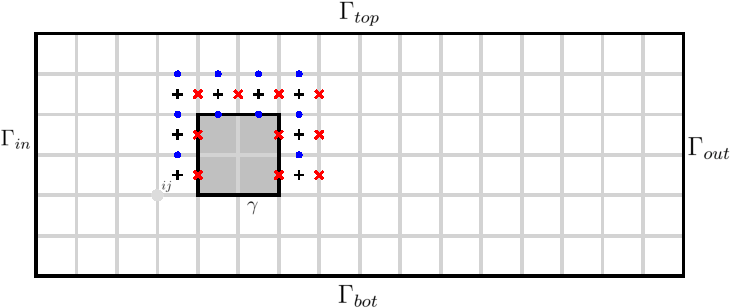
\includegraphics[width=0.8\linewidth]{obstacle_staggered.pdf}
\caption{Область расчёта и разнесённая сетка для задачи обтекания}
\label{fig:obstacle_staggered}
\end{figure}

По аналогии с \figref{fig:staggered_grid} введём в этой области
прямоугольную сетку (\figref{fig:obstacle_staggered}).

В случае сохранения естестественной нумерации узлов и ячеек сетки
часть их этих пронумерованных ячеек выпадает из области расчёта (попадает внутрь препятствия).
Для таких случаев существует два способа работы с нумерацией:
\begin{itemize}
\item
Можно сохранить естественную нумерацию, при этом часть ячеек пометить
как неактивные (например, введя специальный массив признаков \ename{actnum},
$i$-ый элемент которого равен единице для активной ячейки и нулю для неактивной).
Количество элементов в сеточных векторах тогда будет равно общему количеству
всех ячеек (и активных и неактивных). Но значения этих векторов в неактивных ячейках будут фиктивными (нулями).
\item
Можно нумеровать лишь активные ячейки (и узлы), тем самым
нарушив естественную нумерацию. 
\end{itemize}

Оба этих подхода имеют свои очевидные плюсы и минусы.
Первый подход сохраняет простые зависимости для перевода двумерного индекса в сквозной и
диагональную структуру сеточных матриц. Второй подход более экономичен в хранении данных. 

\subsubsection{Граничные условия}
Рассмотрим постановку со следующими граничными условиями:
\begin{itemize}
\item
во входном сечении зададим равномерный профиль скорости
\begin{equation}
\label{eq:ns2d_obstable_bc_in}
(x, y) \in \Gamma_{in}: u=1, \; v=0;
\end{equation}
\item
на нижней и верхней границах -- условие симметрии (идеального скольжения). Это условие моделирует
зеркальное отражение расчётной области относительно соответствующих границ $\Gamma_{top}, \Gamma_{bot}$.
\begin{equation}
\label{eq:ns2d_obstable_bc_topbot}
(x, y) \in \Gamma_{top}, \Gamma_{bot}: \dfr{u}{n}=0, \; v = 0;
\end{equation}
\item
на самом обтекаемом деле -- условия прилипания
\begin{equation}
\label{eq:ns2d_obstable_bc_wall}
(x,y) \in \gamma: u=0, \; v=0;
\end{equation}
\item
в выходном сечении -- условия выхода потока. Их точную формулировку определим позднее.
\end{itemize}

На каждом шаге алогоритма SIMPLE требуется
решить три дифференциальных уравнения \cref{eq:ns2d_ustar,eq:ns2d_vstar,eq:ns2d_pstroke_diff}.
относительно неизвестных $u^*, v^*, p'$.
Значит из представленных выше граничных условий требуется
выразить граничные значения для этих трёх неизвестных сеточных векторов
и расписать способ их учёта при сборке соответствующих систем линейных уравнений.

\subsubsubsection{Входное сечение}
\label{sec:obstacle_bc_input}
При разложении скорости на пробное значение и поправку \cref{eq:ns2d_decomp}
условия для скорости \cref{eq:ns2d_obstable_bc_in} раскладываются следующим образом:
\begin{equation}
\label{eq:ns2d_decomp_input}
(x,y) \in \Gamma_{in}: u^* = 1, \; v^* = 0, \; u' = v' = 0
\end{equation}
Условия первого рода для пробной скорости учитываются при решении уравнений
\cref{eq:ns2d_ustar,eq:ns2d_vstar}.
Для сеточного вектора $u^*$, узлы которого лежат непосредственно на границе,
учёт этого условия сводится к модификации соответствующей строки матрицы $A^u$ и правой части $b^u$.
В строке $k=k\left[0, j+\tfrac12\right]$:
\begin{equation}
\label{eq:ns2d_au_bc_left}
A^u_{km} = \delta_{km}, \quad b^u_k = 1.
\end{equation}

Для сеточного вектора $v^*$ учёт производится с помощью выражения для значения в фиктивном узле $k_1 = k\left[-\tfrac12, j\right]$
через значение в настоящем узле $k_0 = k\left[\tfrac12, j\right]$:
$$
\frac{v^*_{k_0} + v^*_{k_1}}{2} = 0 \hence v^*_{k_1} = -v^*_{k_0}.
$$
Поэтому при сборке матрицы $A^v$ по формулам \cref{eq:ns2d_av} при необходимости добавить
значение $a$ в колонку, соответствующую фиктивному узлу, требуется добавить это значение
в диагональ с обратным знаком:
\begin{equation}
\label{eq:ns2d_av_bc_left}
A^v_{k_0, k_1} {{+}{=}} a \hence A^v_{k_0, k_0} \minuseq a
\end{equation}

Из условий на поправку скорости $u'=v'=0$ и уравнений \cref{eq:ns2d_ustroke_approx,eq:ns2d_vstroke_approx}
следует граничное условие для поправки давления
\begin{equation}
\label{eq:ns2d_obstacle_bc_pres}
x,y\in\Gamma_{in}: \dfr{p'}{x}=0
\end{equation}
Из этого условия получаем соотношение для давления в фиктивном узле $k_1 = k\left[-\tfrac12, j+\tfrac12\right]$
через значение  в реальном узле $k_0 = k\left[\tfrac12, j+\tfrac12\right]$:
$$
p'_{k_1} = p'_{k_0}
$$
Тогда добавление значения $a$ в фиктивную колонку $k_1$ эквивалентно
\begin{equation}
\label{eq:ns2d_ap_bc}
A^p_{k_0, k_1} {{+}{=}} a \hence A^p_{k_0, k_0} \pluseq a
\end{equation}

Следует понимать, что выражение \cref{eq:ns2d_ustroke_approx}
является приближением, используемым в расчётной схеме SIMPLE.
В действительности, использование условия \cref{eq:ns2d_obstacle_bc_pres} (в случае нулевого начального приближения давления)
приводит к нулевой производной для всего давления (а не только поправки)
$$
x,y\in\Gamma_{in}: \dfr{p}{x}=0.
$$
Это выражение никак не следует из постановки задачи.
Действительно, если расписать уравнение \cref{eq:ns2d_u} с учётом условий \cref{eq:ns2d_obstable_bc_in}
и уравнения неразрывности \cref{eq:ns2d_div}, то получим соотношение
\begin{equation}
\label{eq:ns2d_obstacle_true_bc_p}
x,y\in\Gamma_{in}: \dfr{p}{x} = \frac{1}{\Ren}\dfrq{u}{x} = -\frac1\Ren\dfr{}{x}\left(\dfr{v}{y}\right).
\end{equation}
(при выводы учтено, что $\dsfr{v}{y} = -\dsfr{u}{x} = 0$).
Однако, практика показывает, что в большинстве случаев, условий типа \cref{eq:ns2d_obstacle_bc_pres}
оказывается достаточно. Выражение \cref{eq:ns2d_obstacle_true_bc_p} равно нулю,
если поперечная компонента скорости не появляется сразу за входным сечением. То есть
течение остается прямолинейным на начальном участке расчётной области.
Чтобы это исполнялось, входное сечение необходимо размещать
на таком растоянии от препятствия, на котором поток еще не чувствует его присутствия (не начинает разворачиваться).

\subsubsubsection{Условия симметрии}
Однородные условие для скорости \cref{eq:ns2d_obstable_bc_topbot} расписываются
как
$$
(x,y) \in \Gamma_{in}: \dfr{u^*}{y} = \dfr{u'}{y} = 0, \; v^* = v' = 0.
$$
Из условия на $u^*$ запишем соотношение для фиктивного узла около нижней границы, которое будем использовать
при сборке матрицы $A^u$:
\begin{align*}
&k_0 = k\left[i+\tfrac12, \tfrac12\right], \quad k_1 = k\left[i+\tfrac12, -\tfrac12\right], \\
&u^*_{k_1} = u^*_{k_0}, \\
&A^u_{k_0, k_1} {{+}{=}} a \hence A^u_{k_0, k_0} \pluseq a.
\end{align*}
Условие на $v^*$ можно использовать явно:
\begin{align*}
&k = k\left[i+\tfrac12, \tfrac12\right], \\
&A^u_{k,s} = \delta_{ks}, \quad b^u_k = 0.
\end{align*}

Граничное условие для поправки давления
можно получить из уравнения движения \cref{eq:ns2d_v} (в неконсервативном виде) с учётом уравнения неразрывности.
Используя
\begin{align*}
&(x,y) \in \Gamma_{top,bot}:
	v = 0 \hence \dfr{v}{x} = 0 \hence \dfrq{v}{x} = 0,\\
&\phantom{(x,y) \in \Gamma_{top,bot}}:
	\dfr{u}{y} = 0 \hence \dfr{}{x}\dfr{u}{y} = 0 \hence \dfrq{v}{y} = 0,\\
\end{align*}
получим
$$
(x,y) \in \Gamma_{top,bot}: \dfr{p}{y} = 0.
$$
При использовании нулевого начального приближения давления, для поправки давления так же справедливо
$$
(x,y) \in \Gamma_{top,bot}: \dfr{p'}{y} = 0.
$$
Учёт этого условия на матричном уровне аналогичен процедуре \cref{eq:ns2d_ap_bc}.

\subsubsubsection{Условия прилипания}
\label{sec:obstacle-noslip}
Учёт условий прилипания на границе обтекаемого тела \cref{eq:ns2d_obstable_bc_wall}
в целом аналогичен алгоритму учёта входной границы.
Для компонент скорости, узлы которых лежат на границе работает процедура \cref{eq:ns2d_au_bc_left} (с нулём в правой части).
В случае если узлы не лежат на границе, то используется процедура \cref{eq:ns2d_av_bc_left}.

Для поправки давления так же используется однородное условие второго рода \cref{eq:ns2d_obstacle_bc_pres}
И все комментарии к этому условию, указанные в пункте \ref{sec:obstacle_bc_input}, остаются справедливыми.

\subsubsubsection{Выходные граничные условия}
На выходной границе отсутствует возможность указать какие-либо физичные условия для искомых переменных.
При этом, как правило, поведение течения в этой области большого интереса не представляет.
Поэтому здесь требуется написать такие выражения, учёт которых
не оказывал бы влияния на течение в основной области расчёта.
Отсюда возникает проблема формулировки неотражающих граничных условий.
Цель состоит в том, чтобы жидкость выходила из области расчёта естественным для себя образом, не подстраиваясь под выходную границу.

Простейшим решением этой проблемы является использование уравнения переноса на выходной границе:
\begin{equation}
\label{eq:ns2d_outflow_common}
\begin{aligned}
(x,y)\in\Gamma_{out}:\; &\dfr{u}{t} + u\dfr{u}{x} = 0,\\[10pt]
                        &\dfr{v}{t} + u\dfr{v}{x} = 0.
\end{aligned}
\end{equation}
В стационарном случае ($\dsfr{u,v}{t} = 0$) из этих условий следует, что поперечная скорость равна нулю:
\begin{equation*}
\dfr{u}{x} = 0 \hence \dfr{v}{y} = 0 \hence v = v|_{\Gamma_{bot}} = 0.
\end{equation*}

По аналогии с уравнениями движения \cref{eq:ns2d_semi_u}
в уравнение на выходной границе так же добавим фиктивную производную по времени.
Тогда условия для компонент скорости на итерации SIMPLE примут вид (для стационарного случая)

\begin{equation}
\label{eq:ns2d_outflow_common_semi}
\begin{aligned}
(x,y)\in\Gamma_{out}:\; &\frac{\hat u - u}{\tau} + u\dfr{\hat u}{x} = 0,\\[10pt]
                        &\hat v = 0.
\end{aligned}
\end{equation}

Подставим разложение \cref{eq:ns2d_decomp} и запишем условия для уравнений пробной скорости

\begin{align}
\label{eq:ns2d_outflow_ustar}
(x,y)\in\Gamma_{out}:\; &u^* + \tau u\dfr{u^*}{x} = u,\\[10pt]
\label{eq:ns2d_outflow_vstar}
                        &v^* = 0.
\end{align}

Пробная скорость в алгоритме SIMPLE не удовлетворяет уравнению неразрывности.
Поэтому нет гарантий, что найденная $u^*$ сохраняет баланс масса в расчётной области.
На практике это означает, что количество жидкости, которое втекает через $\Gamma_{in}$ не равно
количеству жидкости, которое вытекает через $\Gamma_{out}$.

Но финальная по итогам SIMPLE итерации скорость должна сохранять баланс массы.
То есть
$$
\triangle Q = \int_{\Gamma_{in}} \hat u \, ds - \int_{\Gamma_{out}} \hat u \, ds = 0.
$$
Раскладывая это выражение через пробную скорость и поправку с учётом нулевого значения $u'$ на входной границе \cref{eq:ns2d_decomp_input},
получим
$$
\int_{\Gamma_{out}} u' \, ds = \int_{\Gamma_{in}} u^* \, ds - \int_{\Gamma_{out}} u^* \, ds
$$
Положим, что $u'$ на выходной границе постоянна.
Это предположение не влияет на итоговый результат SIMPLE итераций, так как
при его сходимости поправки скорости обнуляются. Тогда запишем значение поправки скорости
на выходной границе
\begin{equation}
\label{eq:ns2d_ustroke_from_balance}
(x,y)\in\Gamma_{out}:\; u' = \left(\int_{\Gamma_{in}} u^* \, ds - \int_{\Gamma_{out}} u^* \, ds \right) / \left|\Gamma_{out}\right|
\end{equation}
Подставляя это выражение в \cref{eq:ns2d_ustroke_approx}, получим граничные условия на поправку давления
\begin{equation}
\label{eq:ns2d_outflow_pstroke}
(x,y)\in\Gamma_{out}:\;  d^u\dfr{p'}{x} = -\frac{u'}{\tau}
\end{equation}

Таким образом, мы вывели граничные условия для всех трёх дифференциальных уравнений:
\cref{eq:ns2d_outflow_ustar,eq:ns2d_outflow_vstar,eq:ns2d_outflow_pstroke}.

Отметим, что если выходных границ несколько, то выражение \cref{eq:ns2d_ustroke_from_balance}
следует записывать для каждой из границ. При этом следует дополнительно задавать
долю расхода $C_i$, вытекающую через каждую из границ. Пусть $\Gamma_{out} = \Gamma_{o1} \cap \Gamma_{o2}$.
Тогда
\begin{align*}
&(x,y)\in\Gamma_{o1}:\; u' = \left(C_1 \int_{\Gamma_{in}} u^* \, ds - \int_{\Gamma_{o2}} u^* \, ds \right) / \left|\Gamma_{o1}\right|\\
&(x,y)\in\Gamma_{o2}:\; u' = \left(C_2 \int_{\Gamma_{in}} u^* \, ds - \int_{\Gamma_{o1}} u^* \, ds \right) / \left|\Gamma_{o2}\right|\\
&C_1 + C_2 = 1.
\end{align*}

\paragraph{Учёт условия для $u^*$ \cref{eq:ns2d_outflow_ustar}}
Просто перепишем уравнение в строках СЛАУ, соответствующих выходным узлам $k_0 = k\left[n_x, j+\tfrac12\right]$.
Для этого аппроксимируем конвективную производную по схеме против потока (с противопоточным узлом
$k_1 = k\left[n_x-1, j+\tfrac12\right]$).
$$
u^*_{k_0} + \tau U_{k_0} \frac{u^*_{k_0} - u^*_{k_1}}{h_x} = u_{k_0},
$$
где $U$ - скорость переноса в $k_0$-ом узле. Она должна быть всегда больше нуля (иначе схема
перестаёт быть противопотоковой). Можно просто положить её равной среднерасходной (единице в нашем случае).
А можно взять из предыдущей итерации с проверкой на положительность:
$$
U_{k_0} = \max\left(0, u_{k_0}\right).
$$
На матричном уровне получим:
\begin{equation}
\label{eq:ns2d_outflow_ustar_mat}
\begin{aligned}
&A^u_{k0, s} = \begin{cases}
	1 + \dfrac{\tau U_{k_0}}{h_x}, \quad s = k_0\\[10pt]
	-\dfrac{\tau U_{k_0}}{h_x}, \quad s = k_1\\[10pt]
	0, \quad \text{иначе},
\end{cases}, \\
&b^u_{k_0} = u_{k_0}
\end{aligned}
\end{equation}

\paragraph{Учёт условия для $v^*$ \cref{eq:ns2d_outflow_vstar}}
будем осуществлять за счёт введения фиктивного узла:
\begin{align*}
&k_0 = k\left[n_x - \tfrac12, j\right], \; k_1 = k\left[n_x + \tfrac12, j\right], \\
&\frac{v^*_{k_0} + v^*_{k_1}}{2} = v^*_{\Gamma_{out}} = 0 \hence v^*_{k_1} = -v^*_{k_0}.
\end{align*}
Отсюда добавление элемента $a$ в фиктивную колонку будет осуществляться в виде
$$
A^v_{k_0, k_1} \pluseq a \hence A^v_{k_0, k_0} \minuseq a.
$$


\paragraph{Учёт условия для $p'$ \cref{eq:ns2d_outflow_pstroke}}
Также введём фиктивный узел $k_1$ и расположенные левее от него реальный узел $k_0$:
\begin{equation*}
k_0 = k\left[n_x - \tfrac12, j+\tfrac12\right], \; k_1 = k\left[n_x + \tfrac12, j+\tfrac12 \right], \\
\end{equation*}
Из \cref{eq:ns2d_outflow_pstroke}
\begin{equation*}
d^u \frac{p'_{k_1} - p'_{k_0}}{h_x} = -\frac{u'}{\tau} \hence p'_{k_1} = p'_{k_0} -\frac{h_x}{\tau d^u} u'
\end{equation*}
На матричном уровне добавление фиктивной колонки даёт
\begin{equation}
\label{eq:ns2d_outflow_pstrike_mat}
A^v_{k_0, k_1} \pluseq a \hence A^v_{k_0, k_0} \pluseq a, \; b^v_{k_0} \pluseq a \frac{h_x u'}{\tau d^u}.
\end{equation}

\subsubsection{Баланс сил. Коэффициенты сил}

\subsubsubsection{Сопротивление}
Проинтегрируем уравнение движения 
\cref{eq:ns2d_u}
по области расчёта $D$:
$$
\arint{\dfr{u^2}{x}}{D}{\vec x} +
\arint{\dfr{uv}{y}}{D}{\vec x} =
-\arint{\dfr{p}{x}}{D}{\vec x} + \frac{1}{\Ren} \arint{\nabla^2 u}{D}{\vec x}.
$$
Интегрирование по частям даёт:
\begin{align*}
&\arint{\dfr{f}{x}}{D}{\vec x} = \arint{f}{\Gamma_{out}}{s} - \arint{f}{\Gamma_{in}}{s} + \arint{f n_x}{\gamma}{s} \\[10pt]
&\arint{\dfr{f}{y}}{D}{\vec x} = \arint{f}{\Gamma_{top}}{s} - \arint{f}{\Gamma_{bot}}{s}+ \arint{f n_y}{\gamma}{s}, \\[10pt]
&\arint{\nabla^2 f}{D}{\vec x} = \arint{\dfr{f}{n}}{\Gamma}{s} + \arint{\dfr{f}{n}}{\gamma}{s}, \quad \Gamma = \Gamma_{in} \cap \Gamma_{out} \cap \Gamma_{bot} \cap \Gamma_{top}
\end{align*}
Учтём, что на обтекаемом теле скорости равны нулю, а верхняя и нижняя границы непротекаемы.
Тогда
$$
\arint{\left(u^2 + p\right)}{\Gamma_{in}}{s}
-\arint{\left(u^2 + p\right)}{\Gamma_{out}}{s} =
\arint{p \, n_x}{\gamma}{s} - \frac1\Ren\arint{\dfr{u}{n}}{\gamma}{s}
$$
Полученное выражение есть баланс сил в $x$ направлении.
Слева стоит сила, обусловленная перепадом динамического давления
(если считать профили скорости на входе и на выходе примерно одинаковыми, то останется только перепад статического давления).
А справа - силы сопротивления потоку вследствии наличия препятствия. И эти силы уравнавешивают друг друга.
Первое слагаемое в правой части -- есть сопротивление формы, второе -- сопротивление трения из-за эффектов вязкости.

Коэффициенты этих сил имеют следующее выражение:
\begin{equation}
\label{eq:ns2d_cx}
\begin{array}{lll}
	C^p_x =& 2 \displaystyle\arint{p\,n_x}{\gamma}{s} & \text{-- коэффициент сопротивления формы} \\[20pt]
	C^f_x =& -\dfrac2\Ren \displaystyle\arint{\dfr{u}{n}}{\gamma}{s} & \text{-- коэффициент сопротивления трения} \\[20pt]
	C_x =& C^p_x + C^f_x & \text{-- коэффициент сопротивления}
\end{array}
\end{equation}

Чтобы из этих безразмерных коэффициентов получить реальные силы, измеряемые в Ньютонах, нужно умножить их на $\tfrac12 \rho U^2 L^2$.

\subsubsubsection{Подъёмная сила}

Аналогично проинтегрируем уравнение движение в направлении $y$
\cref{eq:ns2d_v}. С учётом граничных условий получим выражение для баланса сил в поперечном направлении
$$
\arint{p}{\Gamma_{bot}}{s}
-\arint{p}{\Gamma_{top}}{s} =
\arint{p \, n_y}{\gamma}{s} - \frac1\Ren\arint{\dfr{v}{n}}{\gamma}{s}
$$
и соответствующие коэффициенты
\begin{equation}
\label{eq:ns2d_cy}
\begin{array}{lll}
	C^p_y =& 2 \displaystyle\arint{p n_y}{\gamma}{s} & \text{} \\[20pt]
	C^f_y =& -\dfrac2\Ren \displaystyle\arint{\dfr{v}{n}}{\gamma}{s} & \text{} \\[20pt]
	C_y =& C^p_y + C^f_y & \text{-- коэффициент подъёмной силы}
\end{array}
\end{equation}

\subsubsubsection{Вычисление коэффициентов сил на разнесённой сетке}
\label{sec:compute-obstacle-coefs}
Вычисления коэффициентов $C_x, C_y$ по формулам \cref{eq:ns2d_cx,eq:ns2d_cy}
сводятся к интегрированию давления и производных скорости по поверхности обтекаемого тела.
Само вычисление интеграла происходит простым суммированием:
\begin{equation}
\label{eq:ns2d_gamma_quadrature}
\arint{f}{\gamma}{s} \approx \sum_i f_i |\gamma_i|,
\end{equation}
где $\gamma_i$ -- отрезок границы поверхности $\gamma$, а $f_i$ -- значение функции в центре этого отрезка.
В случае равномерной сетки $|\gamma_i| = h_x, h_y$ для горизонтальных и вертикальных отрезков соответственно.
Задача сводится к определению значению функций $p$, $\dsfr{u,v}{n}$ в центрах отрезков.

\paragraph{Горизонтальная граница} Зафиксируем узел $i+\tfrac12, j$ на такой границе.
На этой границе $n_x$ равна нулю, и вклад в $C^p_x$ он не даёт.
Для вычисления вклада в $C^f_x$ нужно вычислить $\dsfr{u}{y}$.
Для верхней границе запишем:
\begin{align*}
&u_{i+\tfrac12, j} = 0 \quad \text{из граничных условий прилипания},\\
&u_{i+\tfrac12, j + \tfrac12} = \frac{u_{i, j+\tfrac12} + u_{i+1, j + \tfrac12}}{2}
\end{align*}
отсюда
\begin{equation*}
\dfr{u}{n} =
-\dfr{u}{y} = \frac{u_{i+\tfrac12, j} - u_{i+\tfrac12, j+\tfrac12}}{h_y/2} =
              -\frac{u_{i, j+\tfrac12} + u_{i+1, j + \tfrac12}}{h_y}
\end{equation*}
Аналогично для нижней границы
\begin{equation*}
\dfr{u}{n} =
\dfr{u}{y} =
\frac{u_{i+\tfrac12, j} - u_{i+\tfrac12, j-\tfrac12}}{h_y/2} =
-\frac{u_{i, j-\tfrac12} + u_{i+1, j - \tfrac12}}{h_y}
\end{equation*}

Для вычисления вклада в $C_y^p$ необходимо определить давление в $i+\tfrac12, j$.
На границе $\gamma$ мы использовали условие $\dsfr{p}{n} = 0$ (см п. \ref{sec:obstacle-noslip}).
Отсюда на верхней границе:
\begin{equation*}
\dfr{p}{n} = \frac{p_{i+\tfrac12, j} - p_{i+\tfrac12, j+\tfrac12}}{h_y} = 0
\hence p_{i+\tfrac12, j} = p_{i+\tfrac12, j+\tfrac12}.
\end{equation*}
Тогда подинтегральное выражение равно
\begin{equation*}
p\,n_y = -p_{i+\tfrac12, j+\tfrac12}
\end{equation*}
Аналогично на нижей границе получим:
\begin{equation*}
p\,n_y = p_{i+\tfrac12, j-\tfrac12}
\end{equation*}

Вклад горизонтальной границы в коэффициент $C^f_y$
вычисляется через значение $\dsfr{v}{y}$, которое равно нулю из-за условий прилипания.

\paragraph{Вертикальная граница}
Теперь зафиксируем узел $i, j+\tfrac12$ на вертикальной границе.
Вклад этой границы в коэффициенты $C^p_y, C^f_x$ равны нулю:
первого из-за значения $n_y$, а второго из-за $\dsfr{u}{x} = -\dsfr{v}{y} = 0$.

Для коэффициента $C^p_x$ напишем:
\begin{equation}
\label{eq:ns2d_obstacle_pnx_vertical}
\begin{aligned}
& p\,n_x = p_{i-\tfrac12, j+\tfrac12} \quad \text{-- левая граница},\\
& p\,n_x = -p_{i+\tfrac12, j+\tfrac12} \quad \text{-- правая граница}.
\end{aligned}
\end{equation}

Для $C^f_y$:
\begin{equation}
\label{eq:ns2d_obstacle_dvdn_vertical}
\begin{aligned}
& \dfr{v}{n} = - \frac{v_{i-\tfrac12, j} + v_{i-\tfrac12, j+1}}{h_x} \quad \text{-- левая граница},\\
& \dfr{v}{n} = - \frac{v_{i+\tfrac12, j} + v_{i+\tfrac12, j+1}}{h_x} \quad \text{-- правая граница}.
\end{aligned}
\end{equation}


\subsection{Задание для самостоятельной работы}

В SIMPLE-решателе для течения вязкой жидкости в каверне \cvar{[cavern2-simple]}
рассмотреть
простые итерационные подходы к решению систем уравнений
для $u^*$, $v^*$:
\begin{itemize}
\item метод Якоби (\ref{sec:SLAE-Jacobi}),
\item метод Зейделя (\ref{sec:SLAE-Seidel}),
\item метод SOR (\ref{sec:SLAE-SOR}).
\end{itemize}

Реализовать означенные решатели в виде функций вида:
\begin{minted}[linenos=false]{c++}
// Single Jacobi iteration for mat*u = rhs SLAE. Writes result into u
void jacobi_step(const cfd::CsrMatrix& mat, const std::vector<double>& rhs, std::vector<double>& u){
    ...
\end{minted}
которые делают одну итерацию соответствующего метода без проверок на сходимость.
Аргумент \cvar{u} используется как начальное значение искомого сеточного вектора. Туда же пишется 
итоговый результат.

Эти функции необходимо вызывать вместо
\begin{minted}[linenos=false]{c++}
AmgcMatrixSolver::solve_slae
\end{minted}
в соответствующих решателях
\cvar{Cavern2DSimpleWorker::compute_u_star},
\cvar{Cavern2DSimpleWorker::compute_v_star}.

Если требуется сделать несколько шагов, то вызывать несколько раз подряд.


Все алгоритмы основаны на вычислении выражения вида
\begin{equation*}
   \frac{1}{A_{ii}}\left(r_i - \sum_{j=0}^{N-1} A_{ij}{u_j}\right),
\end{equation*}
поэтому рекомендуется выделить отдельную функцию, которая бы вычисляла это выражение
и использовалась всеми тремя решателями
\begin{minted}[linenos=false]{c++}
double row_diff(size_t irow, const cfd::CsrMatrix& mat, const std::vector<double>& rhs, const std::vector<double>& u){
	const std::vector<size_t>& addr = mat.addr();   // массив адресов
	const std::vector<size_t>& cols = mat.cols();   // массив колонок
	const std::vector<double>& vals = mat.vals();   // массив значений
    ...
}
\end{minted}

Использовать параметры решателя:
\begin{equation*}
    \Ren = 100, \quad E = 4, \quad n_x = n_y = 50, \quad \eps = 10^{-2}.
\end{equation*}

Сделать замеры времени исполнения:
\begin{itemize}
\item \ename{total} -- общее время работы итераций SIMPLE,
\item \ename{assemble} -- время сборки систем уравнений для $u^*$, $v^*$,
\item \ename{p-solver} -- время решения системы для $p'$,
\item \ename{uv-solvers} -- время решения систем для $u^*$, $v^*$.
\end{itemize}

Замеры проводить в Release-версии сборки и с отключенными функциями сохранения в vtk.

Для замера времени исполнения участка кода воспользоваться функциями
\begin{itemize}
\item \cvar{cfd::dbg::Tic} -- вызвать до начала участка кода
\item \cvar{cfd::dbg::Toc} -- вызвать после окончания участка кода
\end{itemize}

Так, чтобы замерить время \ename{total}, нужно обрамить SIMPLE - цикл следующими вызовами
\begin{minted}[linenos=false]{c++}
// iterations loop
dbg::Tic("total");   // запустить таймер total
size_t it = 0;
for (it=1; it < max_it; ++it){
    double nrm = worker.step();
    ...
}
dbg::Toc("total");  // остановить таймер total
\end{minted}

Замеры времени p-solver и uv-solver делать в функции \cvar{Cavern2DSimpleWorker::step}:
\begin{minted}[linenos=false]{c++}
dbg::Tic("uv-solvers");
std::vector<double> u_star = compute_u_star();
std::vector<double> v_star = compute_v_star();
dbg::Toc("uv-solvers");
dbg::Tic("p-solver");
std::vector<double> p_stroke = compute_p_stroke(u_star, v_star);
dbg::Toc("p-solver");
\end{minted}

Замеры времени для сборки левых частей СЛАУ -- в функции \cvar{Cavern2DSimpleWorker::set_uvp}:
\begin{minted}[linenos=false]{c++}
dbg::Tic("assemble");
assemble_u_slae();
assemble_v_slae();
dbg::Toc("assemble");
\end{minted}

При правильном задании функций замеров, по окончанию работы в консоль должен напечататься отчёт о времени исполнения вида:
\begin{shelloutput}
     total:  6.670 sec
uv-solvers:  5.220 sec
  assemble:  1.210 sec
  p-solver:  0.181 sec
\end{shelloutput}

Заполнить таблицу

\begin{equation*}
\begin{array}{l|c|c|c|c|c|c}
    Метод & \text{Кол-во итераций} & \text{Кол-во итераций} & \text{total, s} & \text{assemble, s} & \text{p solver, s} & \text{uv solvers, s}\\
          & \text{решателя СЛАУ}   & \text{SIMPLE}          & & & & \\
    \hline
    \text{Amg} & - &  & & & & \\
    \hline
    \text{Якоби} & 1 &  &  & & & \\
    \hline
    \text{Якоби} & 2 &  &  & & &\\
    \hline
    \text{Якоби} & 4 &  &  & & &\\
    \hline
    \text{Зейдель} & 1 &  &  & & &\\
    \hline
    \text{Зейдель} & 2 &  &  & & &\\
    \hline
    \text{Зейдель} & 4 &  &  & & &\\
    \hline
    \text{SOR} & 1 &  &  & & &\\
\end{array}
\end{equation*}
Здесь Amg - исходный решатель.

Сравнить полученное время исполнения со временем, которое занимает исходный метод.
Подобрать оптимальный с точки зрения времени исполнения метод решения СЛАУ и его настройки (количество внутренних итераций).
